\chapter{تکنولوژی‌های استفاده‌شده}

در این فصل تکنولوژی‌ها و چارچوب\LTRfootnote{Framework}‌های اصلی دخیل در توسعه این دستگاه را به طور دقیق مورد بررسی قرار می‌دهیم.

\section{‌‌زبان برنامه‌نویسی}
برای انتخاب زبان برنامه‌نویسی مناسب برای توسعه مدل یادگیری ماشین شرح‌داده شده، باید معیارهای متفاوتی را در نظر گرفت. برای این منظور زبان پایتون\LTRfootnote{\href{https://docs.python.org/3/}{Python}} را برگزیدیم. مواردی همچون داشتن چارچوب‌ها و کتابخانه‌های قدرتمند یادگیری ماشین، توسعه‌ی آسان و سریع و محبوبیت بالا از دلایل اصلی انتخاب پایتون به عنوان زبان اصلی برای توسعه‌ی سرویس یادگیری ماشین می‌باشد. همچنین شایان ذکر است که چون کارگزار اصلی جمع‌آوری اطلاعات لرزش به زبان پایتون نوشته شده است، استفاده از این زبان برای توسعه مدل یادگیری ماشین، باعث بهبود توسعه‌پذیری نیز می‌گردد. 

\subsection{زبان برنامه‌نویسی پایتون}
یک زبان برنامه‌نویسی عمومی و سطح بالا است که فلسفه طراحی آن بر روی خوانایی کد تأکید دارد. نحو\LTRfootnote{Syntax} پایتون به برنامه‌نویسان امکان می‌دهد تا مفاهیم را با تعداد کمتری خط کد نسبت به زبان‌هایی مانند سی\LTRfootnote{C Programming Language} بیان کنند و این زبان ساختارهایی را فراهم می‌کند که برنامه‌های واضح و قابل فهم را در هر دو مقیاس کوچک و بزرگ فراهم می‌سازد\cite{van2007python}. یکی از مشخصه‌های مهم پایتون این است که از چندین الگو\LTRfootnote{Paradigm}ی برنامه‌نویسی، از جمله شیءگرا\LTRfootnote{Object Oriented Programming (OOP)} و تابعی یا روش‌های رویه‌ای، پشتیبانی می‌کند. پایتون سیستم نوع پویا و مدیریت خودکار حافظه را پشتیبانی می‌کند و کتابخانه‌های استاندارد و جانبی بزرگ و جامع دارد. مفسرهای پایتون برای بسیاری از سیستم‌عامل‌ها در دسترس هستند\cite{srinath2017python}. از جمله مهم‌ترین ویژگی‌های پایتون می‌توان به موارد زیر اشاره کرد.

\begin{itemize}

\item \textbf{سادگی}: پایتون یک زبان برنامه‌نویسی بسیار سطح بالا است که منابع زیادی برای یادگیری آن وجود دارد. پایتون از ابزارهای شخص ثالث متنوعی پشتیبانی می‌کند که استفاده از آن را بسیار آسانتر می‌کند و کاربران را ترغیب می‌کند تا ادامه دهند\cite{srinath2017python, sharma2020python}.

\item \textbf{متن‌باز بودن\LTRfootnote{Open Source}}: اگرچه تمام حقوق این زبان برنامه‌نویسی متعلق به سازمان پایتون است، اما درحال‌ حاضر به عنوان یک نرم‌افزار متن‌باز وجود دارد و هیچ محدودیتی در استفاده، تغییر و توزیع آن وجود ندارد. می‌توان به آزادی از پایتون استفاده کرد و آن را برای استفاده شخصی و یا تجاری توزیع کرد. نه تنها می‌توان نرم‌افزاری که با آن نوشته شده است را استفاده و توزیع کرد، بلکه حتی می‌توان تغییراتی در خود کد منبع پایتون اعمال کرد. همچنین شایان ذکر است که پایتون یک جامعه بزرگ و پویا دارد که در هر نسخه آن را بهبود می‌بخشد\cite{srinath2017python, sharma2020python}.

\item \textbf{کتابخانه‌ها و چارچوب‌ها}: پایتون دارای یک سری کتابخانه‌های استاندارد و چارچوب‌های متنوع است که کار برنامه‌نویسان را بشدت راحت می‌کند، زیرا نیازی نیست تمام کدنویسی را خود برنامه‌نویس انجام دهد. کتابخانه‌های استاندارد در پایتون به خوبی تست شده‌اند و توسط هزاران نفر استفاده می‌شوند. بنابراین، می‌توان اطمینان داشت که استفاده از این کتابخانه‌ها توانایی ایجاد خرابی در برنامه‌های شما را ندارند\cite{srinath2017python, sharma2020python}.

\end{itemize}

حال به بررسی معایب پایتون می‌پردازیم. نکته‌ی قابل توجه در این قسمت این است که اگر معایب نام‌برده شده تاثیر زیادی در کیفیت خدمت ارائه‌شده به کاربر بگذارند، استفاده از پایتون اصلا توصیه نمی‌شود و باید به دنبال جایگزینی مناسب گشت. از جمله کاستی‌های پایتون عبارت‌اند از:

\begin{itemize}

\item \textbf{کندی}: به عنوان یک زبان با نوع پویا، پایتون به دلیل انعطاف‌پذیری بالا، کند عمل می‌کند، زیرا ماشین باید بسیاری از مراجعات را انجام دهد تا از تعریف چیزی مطمئن شود و این باعث کاهش عملکرد پایتون می‌شود\cite{srinath2017python, sharma2020python}.

\item \textbf{دشواری فرایند نگهداری\LTRfootnote{Maintaining}}: به دلیل اینکه پایتون یک زبان با نوع پویا است، یک چیز ممکن است به راحتی به معنای متفاوتی در تک‌نمایی متفاوت تفسیر شود. با افزایش اندازه و پیچیدگی یک برنامه پایتون، نگهداری آن ممکن است دشوار شود. با کمک تست‌های واحد\LTRfootnote{Unit Tests} می‌توان تا حدی این از وقوع این مشکل جلوگیری کرد\cite{srinath2017python, sharma2020python}.

\end{itemize}



\section{چارچوب‌ها و کتاب‌خانه‌ها}
در این پروژه از چارچوب فست‌ای‌پی‌آی\LTRfootnote{\href{https://fastapi.tiangolo.com/}{FastAPI}} برای دریافت درخواست‌ها و ارسال نتایج پیش‌بینی استفاده‌شده است(لوگوی مربوط به این چارچوب در \cref{fig:fastapi_logo}\cite{tiangoloFastAPI} آورده‌شده است). این سرویس به عنوان یک بسته\LTRfootnote{Package}ی پایتونی به کارگزار\LTRfootnote{Server} اصلی اضافه شده است. همچنین برای پیاده‌سازی مدل و انجام محاسبات ریاضی و ماتریسی از کتابخانه‌های نام‌پای\LTRfootnote{\href{https://numpy.org/}{NumPy}} و سایکیت\LTRfootnote{\href{https://scikit-learn.org/}{Scikit-Learn}} بهره برده شده است. در بخش‌های بعد به معرفی مختصر هر کدام از این موارد خواهیم پرداخت. لازم به ذکر است که جهت خوانایی بیشتر، از معادل انگلیسی این کتاب‌خانه‌ها برای اشاره به اسم آنها استفاده خواهیم کرد.

\subsection{چارچوب \lr{FastAPI}}
یک چارچوب مدرن با عملکرد عالی برای طراحی وب است که برای پایتون توسعه داده‌شده است. از ویژگی‌های کلیدی \lr{FastAPI} می‌توان به موارد زیر اشاره کرد\cite{tiangoloFastAPI}.

\begin{figure}[!h]
\centerline{
\includegraphics[width=\textwidth]{fastapi_logo.png}}
\caption{لوگوی \lr{FastAPI}\cite{tiangoloFastAPI}}
\label{fig:fastapi_logo}
\end{figure}
\begin{itemize}

\item \textbf{سریع‌بودن}: همانطور که در قسمت‌های قبل بدان اشاره شده، یکی از معایب پایتون کند بودن می‌باشد. نکته‌ی قابل توجه در اینجا این است که با وجود اینکه یکی از چارچوب‌های پایتون است، اما \lr{FastAPI} بسیار سریع است و کارایی و عملکرد بسیار بالایی را در اختیار می‌گذارد.

\item \textbf{سادگی توسعه}: بدلیل اینکه این زبان از نحو پایتون برای توسعه بهره می‌برد، سرعت توسعه‌دهنده برای ایجاد برنامه را دو تا سه برابر نسبت به چارچوب‌های دیگر برای توسعه برنامه‌ی تحت وب افزایش می‌دهد.

\item \textbf{کوتاه‌بودن}: این ویژگی باعث می‌شود که تکرار کد به حداقل میزان ممکن برسد و این خود منجر به این می‌شود که اشکالات\LTRfootnote{Bugs} کمتری که منشاء آن برنامه‌نویس هستند پیش بیایند.

\end{itemize}

\subsection{کتاب‌خانه‌ی \lr{NumPy}}
\lr{NumPy} یکی از معروف‌ترین کتاب‌خانه‌های زبان پایتون برای پردازش علمی و عددی است و اکنون، ۱۸ سال پس از عرضه، همانطور که در \cref{fig:numpy_related_packs}\cite{van2011numpy} مشخص است، مبنای بسیاری از کتاب‌خانه‌های دیگر پایتون است. این کتاب‌خانه‌ی متن‌باز توسط جامعه‌ی پایتونی توسعه‌یافته است و یک شیء آرایه چندبعدی پایتون به همراه تابع‌هایی که روی آن عمل می‌کنند، ارائه می‌دهد. \lr{NumPy} بدلیل سادگی ذاتی، به عنوان ساختار اصلی مبادله اطلاعات آرایه‌ای در پایتون مورد استفاده قرار می‌گیرد\cite{harris2020array}. آرایه‌ی نام‌پای در واقع یک ساختمان داده است که به صورت بهینه آرایه‌های چند‌بعدی پایتون را ذخیره می‌کند و به آن‌ها دسترسی پیدا می‌کند. همچنین توانایی انجام محاسبات علمی مختلف را بر روی این آرایه‌ها برای ما فراهم می‌کند. این ساختمان داده شامل یک اشاره‌گر\LTRfootnote{Pointer} به حافظه و تعدادی فراداده\LTRfootnote{Metadata} برای تفسیر داده‌های موجود در آرایه است\cite{harris2020array, van2011numpy}.

\begin{figure}[!h]
\centerline{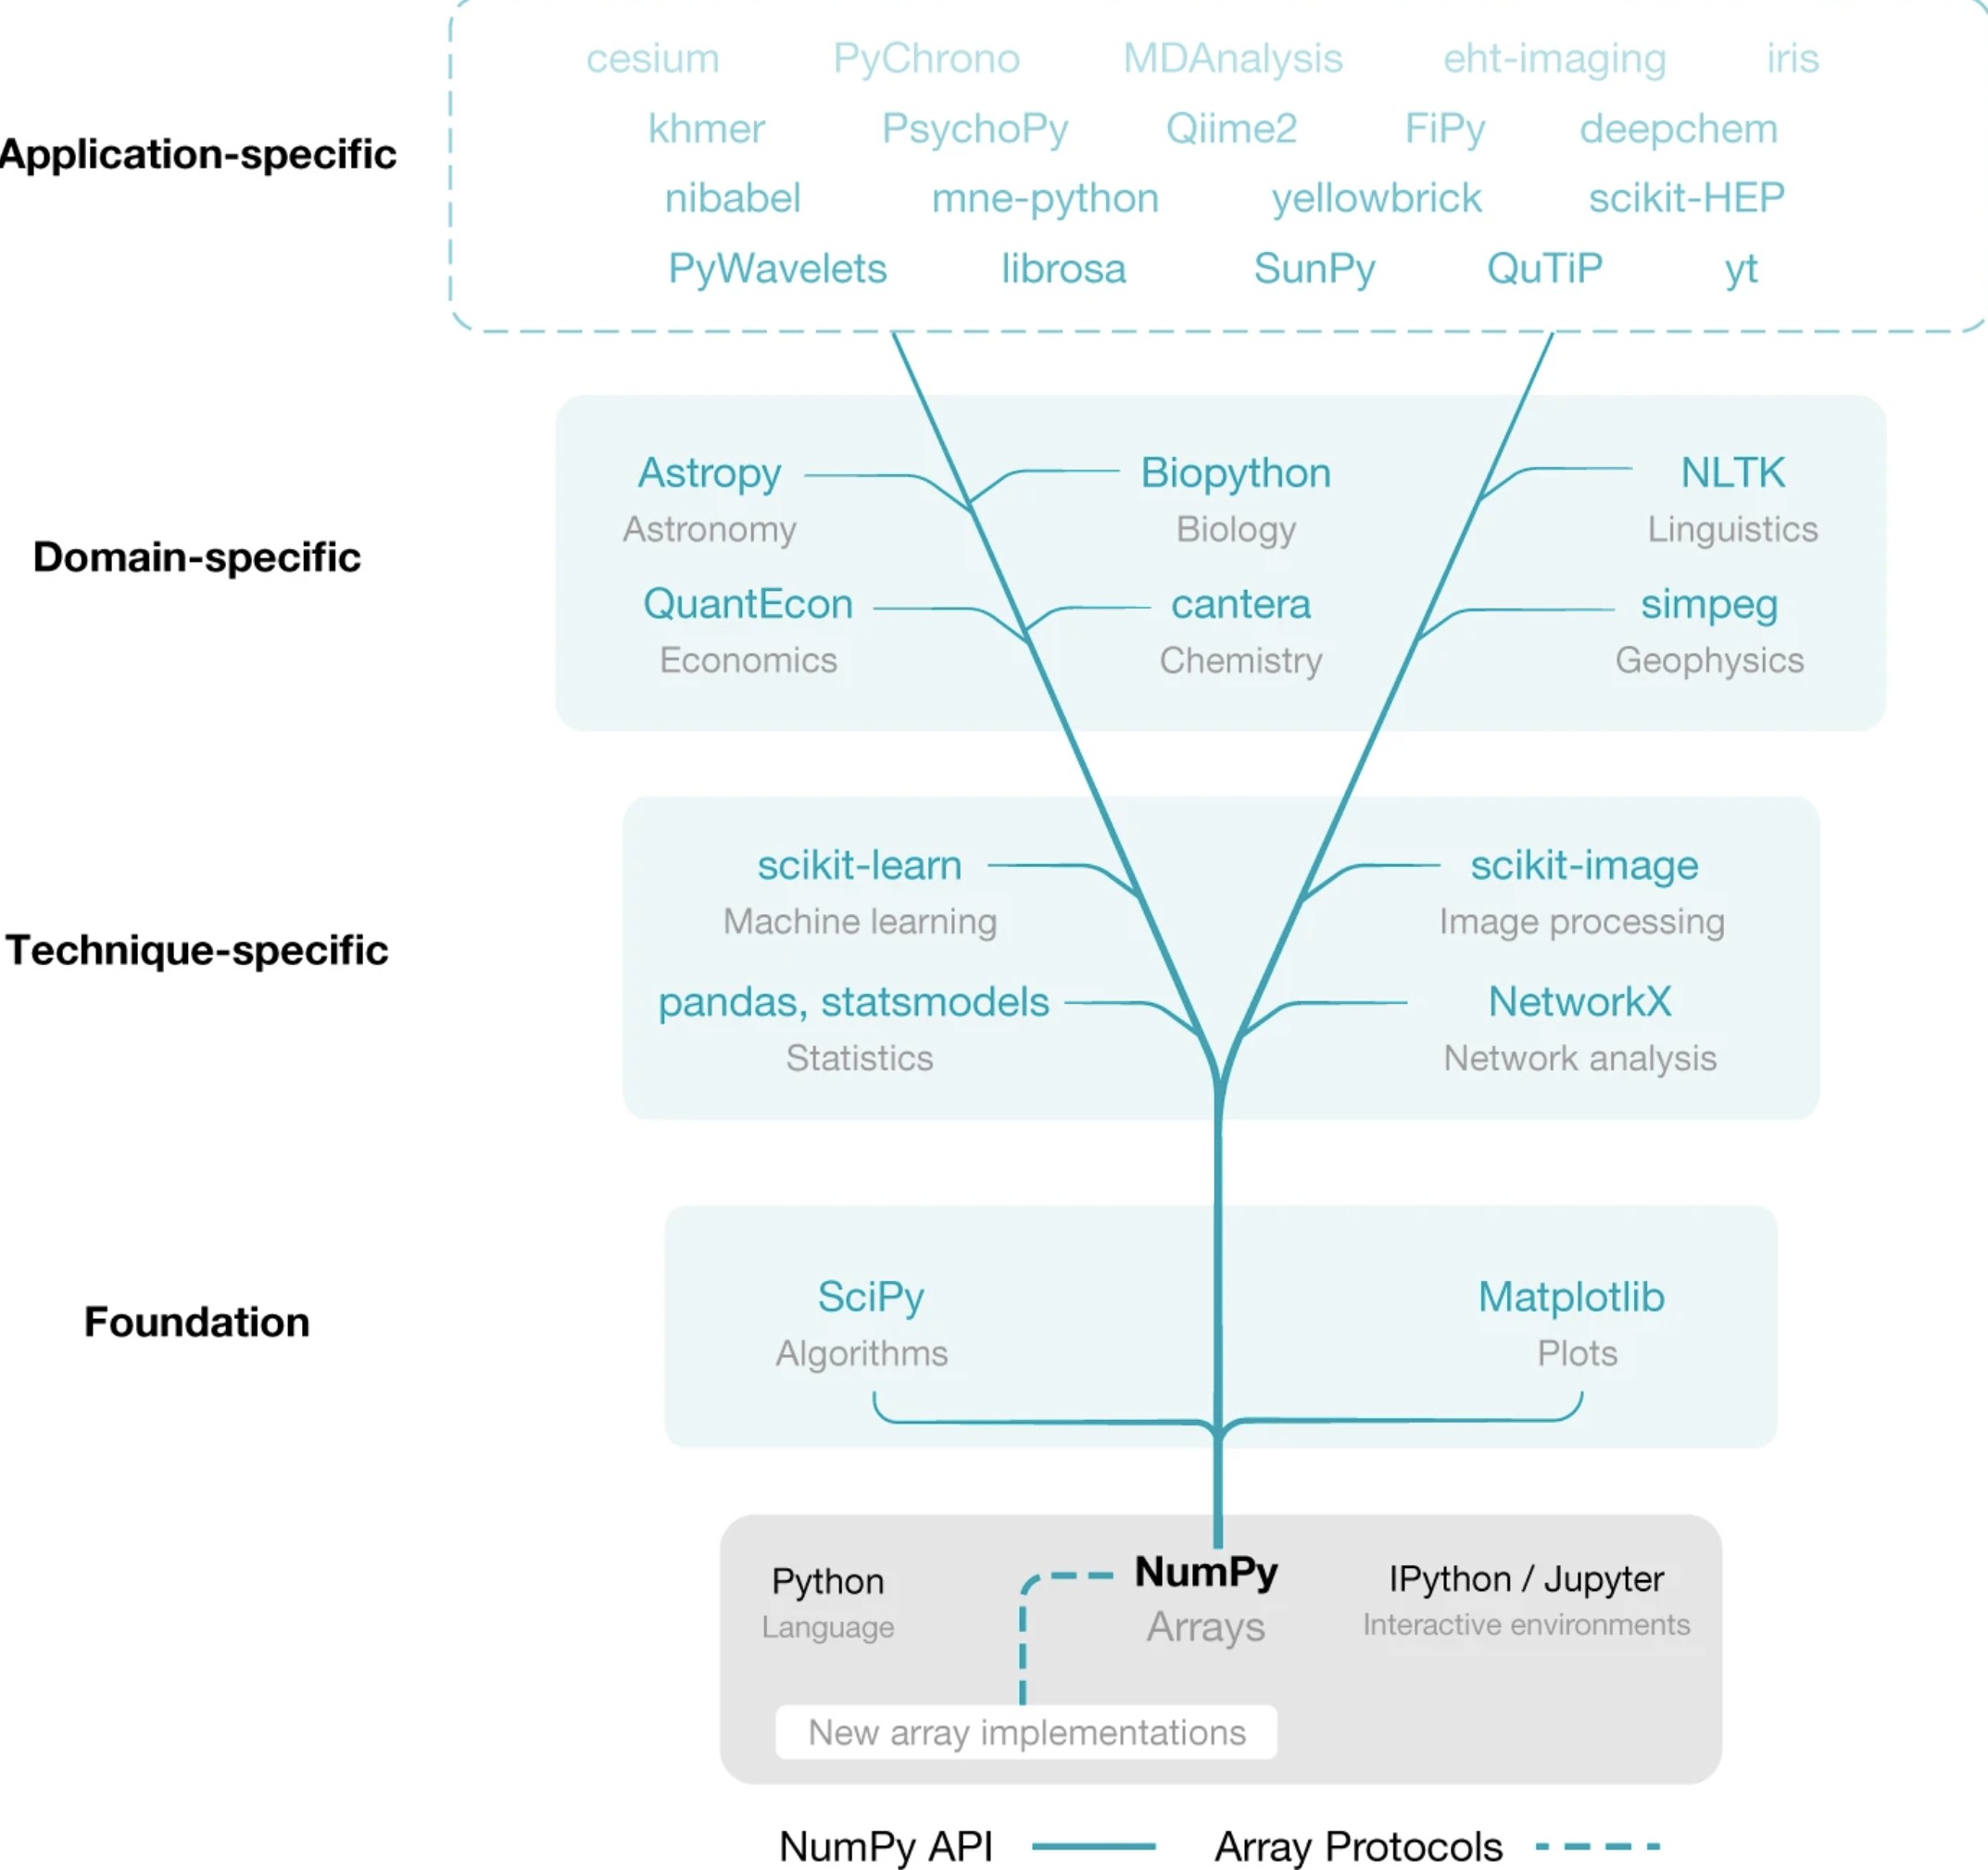
\includegraphics[width=\textwidth]{numpy_related_packs.png}}
\caption{گراف وابستگی کتاب‌خانه‌های پایتون به \lr{NumPy}\cite{van2011numpy}}
\label{fig:numpy_related_packs}
\end{figure}

\subsection{کتاب‌خانه‌ی \lr{Scikit-Learn}} 
\lr{Scikit-Learn}، جامع‌ترین و بزرگ‌ترین بسته یادگیری ماشین منبع‌باز در پایتون است. چون یادگیری ماشین اغلب به عنوان یک جزء از یک برنامه عمومی‌تر (همانند پروژه‌ی کنونی که به عنوان یک سرویس در وب توسعه داده‌شده است) استفاده می‌شود، ایده‌آل است که از همان زبان برنامه‌نویسی استفاده شود تا به‌صورت یکپارچه با سایر بخش‌های برنامه هماهنگ شود. با استفاده از قابلیت‌های گسترده پایتون، \lr{Scikit-Learn} به عنوان یک بسته محبوب برای برنامه‌های مرتبط با یادگیری ماشین در حال رشد است\cite{hao2019machine}. این کتاب‌خانه شامل توابع و اشیاء فراوانی برای مسائل طبقه‌بندی، رگرسیون، تقریب ماتریس کوواریانس، کاهش بعد و پیش‌پردازش داده‌ی خام می‌باشد\cite{kramer2016scikit}. اگرچه پایتون یک زبان برنامه‌نویسی تفسیری است، اما بیشتر روش‌های یادگیری ماشین در \lr{Scikit-Learn} بر پایه کتابخانه‌های دودویی کامپایل شده است که در ابتدا با زبان‌های فورتران\LTRfootnote{Fortran}، سی یا سی‌پلاس‌پلاس\LTRfootnote{C++} برنامه‌نویسی شده‌اند. این پیاده‌سازی‌های مبتنی بر دودویی‌ها به طور قابل توجهی کارایی محاسبات را بهبود می‌بخشند\cite{hao2019machine, kramer2016scikit}.

\section{جمع‌بندی و نتیجه‌گیری}